\subsubsection{Modelo de dominio}

El modelo de dominio representado en la \autoref{fig:domain-model} ilustra las principales entidades y relaciones involucradas en la gestión de un AD, que es la base del sistema propuesto. Este modelo permite comprender las interacciones y dependencias entre los diferentes objetos del sistema.

\begin{figure}[H]
    \centering
    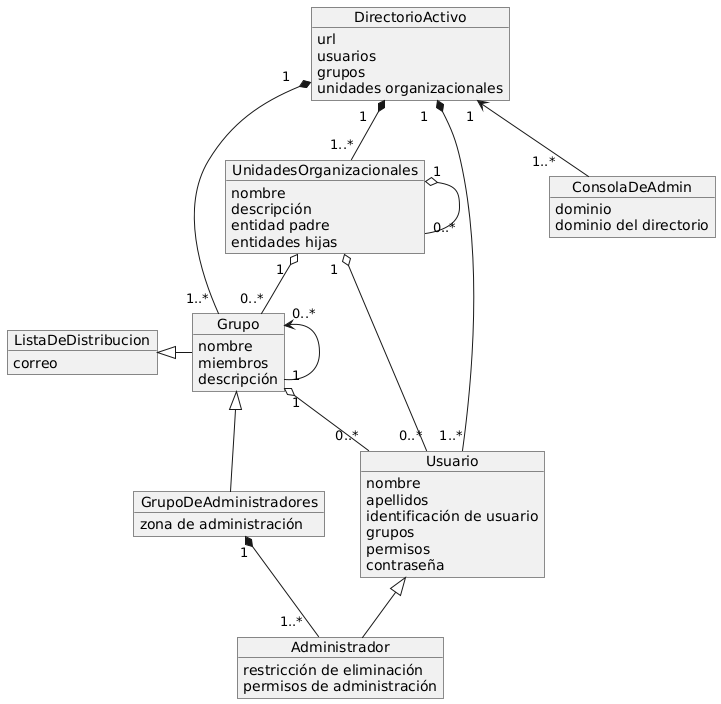
\includegraphics[width=\linewidth]{images/puml/domain-diagram/domain diagram.png}
    \caption{Modelo de dominio del sistema}
    \label{fig:domain-model}
\end{figure}